\chapter{Plataformas de desarrollo}
\label{cap:capitulo3}

En este capítulo se describen en detalle las tecnologías y herramientas empleadas durante el desarrollo de este \ac{TFG}, incluyendo el simulador, las herramientas de percepción, el editor, así como el lenguaje de programación y las librerías utilizadas. Además, se expone el hardware empleado para llevar a cabo los entrenamientos.

\section{Lenguajes de programación}
\label{sec:programación}
\subsection{Python}
\label{sec:python}

Python \footnote{\url{https://www.python.org/}} es un lenguaje de programación de alto nivel \footnote{\url{https://www.tecnologia-informatica.com/lenguaje-de-alto-nivel-que-es-ejemplos/}} interpretado \footnote{\textbf{Lenguaje de programación interpretado}: Lenguaje en el que las implementaciones se ejecutan directamente, sin necesidad de compilar el programa ni generar código máquina del mismo.} que ha ganado gran popularidad en los últimos años gracias a su simplicidad, versatilidad y enfoque multiparadigma \footnote{\textbf{Multiparadigma:} soporta programación orientada a objetos, funcional y procedimental.}. Posee una extensa colección de librerías que facilitan el desarrollo de aplicaciones en áreas muy diversas.

En este \ac{TFG}, Python 3 se emplea para el desarrollo completo del código, utilizando diversas bibliotecas tanto para la creación de entornos de entrenamiento y prueba de modelos, como para la implementación de comportamientos basados en \ac{DRL}.

\subsubsection{Pygame}
\label{sec:pygame}

Pygame \footnote{\url{https://www.pygame.org/docs/}} es una librería de Python ampliamente utilizada para el desarrollo de juegos y aplicaciones multimedia. Proporciona un conjunto de herramientas que permite crear gráficos, visualizar imágenes y gestionar animaciones de manera sencilla y eficiente. Además, Pygame ofrece funcionalidades para la captura y el manejo de eventos de entrada, como las pulsaciones de teclas y los clics del ratón.

\begin{code}[h]
\begin{lstlisting}[language=Python]
import pygame

# Setup
pygame.init()
screen = pygame.display.set_mode(size, pygame.HWSURFACE | pygame.DOUBLEBUF)
pygame.display.set_caption(name)

while True:
	for event in pygame.event.get():
		if event.type == pygame.QUIT:
			pygame.quit()
			break

	screen.fill("purple") # Fill the screen with a color
	pygame.display.flip() # Display your work on the screen
\end{lstlisting}
\caption[Ejemplo de código en Python utilizando Pygame]{Ejemplo de código en Python utilizando Pygame para mostrar una interfaz gráfica}
\label{cod:pygame}
\end{code}

En este caso, se ha utilizado Pygame para desarrollar la interfaz gráfica del proyecto, permitiéndonos visualizar la nube de puntos del \ac{LiDAR} y las imágenes de las cámaras, incluyendo la detección del carril y clasificación de objetos.

\begin{figure}[ht]
\begin{center}
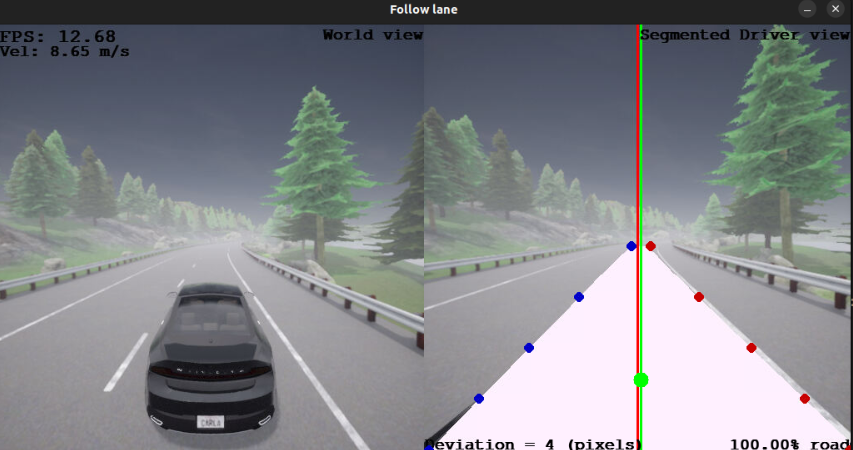
\includegraphics[width=12cm]{figs/Plataformas_Desarollo/pygame.png}
\end{center}
\caption{Interfaz gráfica desarrollada con Pygame donde se visualiza la detección del carril y el \ac{LiDAR}.}
\label{foto_pygame}
\end{figure}

\subsubsection{NumPy}
\label{sec:numpy}

NumPy \footnote{\url{https://numpy.org/}} es una librería de Python que proporciona soporte para matrices y ofrece una extensa colección de funciones matemáticas y operaciones optimizadas para trabajar con estos arreglos. Es ampliamente utilizada por su eficiencia computacional y facilidad de uso. En este proyecto, ha sido muy útil para manejar los \textit{arrays} utilizados para clasificar los puntos del \ac{LiDAR}y las matrices de imágenes y máscaras, permitiéndonos analizar y filtrar estos datos de manera eficiente.

\begin{code}[h]
\begin{lstlisting}[language=Python]
import numpy as np

index = np.argwhere(self._mask == ROAD)
index_sorted = index[np.argsort(index[:, 0])] # Sorted by y

\end{lstlisting}
\caption[Ejemplo de indexación y ordenación de datos con NumPy]{Ejemplo de indexación y ordenación de datos con NumPy}
\label{cod:numpy}
\end{code}

\subsubsection{Matplotlib}
\label{sec:plot}

La librería Matplotlib \footnote{\url{https://matplotlib.org/}} es una herramienta muy popular en Python para crear gráficos y otras visualizaciones. Permite generar todo tipo de diagramas, como líneas, barras o histogramas. Es comúnmente utilizada gracias a su flexibilidad para personalizar los gráficos y su integración con otras librerías como NumPy y Pandas \footnote{\url{https://pandas.pydata.org/}}, librería de Python para la manipulación y análisis de datos. Además, ofrece la posibilidad de exportar los gráficos en diversos formatos. En este \ac{TFG}, se ha utilizado principalmente para la visualización de los datos recopilados durante la inferencia y a lo largo de los entrenamientos.

\begin{code}[h]
\begin{lstlisting}[language=Python]
import matplotlib.pyplot as plt
import matplotlib.patches as mpatches

if points:
	# Scatter plot with colors based on finish
	color_map = {0: 'red', 1: 'green'}
	plt.scatter(range(len(data)), data, color=[color_map[f] for f in finish], s=7)
	
	# Legend
	red_patch = mpatches.Patch(color='red', label='Finish = False')
	green_patch = mpatches.Patch(color='green', label='Finish = True')
	plt.legend(handles=[red_patch, green_patch])  
else:
	plt.plot(range(len(data)), data, linewidth=1, label=key)
	cumulative_avg = np.cumsum(data) / np.arange(1, len(data) + 1)
	plt.plot(range(len(data)), cumulative_avg, label=label, linewidth=2.5)
	plt.legend()

plt.ylabel(key)
plt.xlabel('Episode')
plt.title(title)
\end{lstlisting}
\caption[Ejemplo de código en Python para visualizar datos con Matplotlib]{Ejemplo de código en Python para visualizar datos con Matplotlib.}
\label{cod:plot}
\end{code}

\begin{figure}[ht]
  \begin{center}
    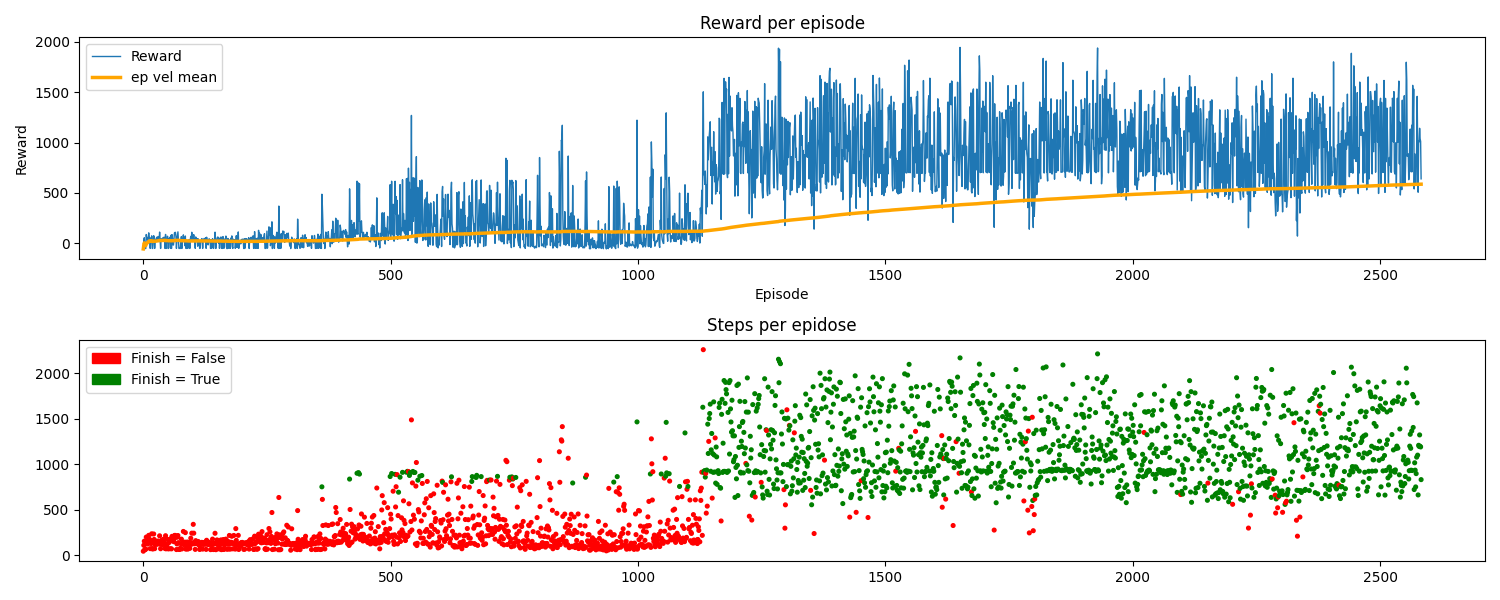
\includegraphics[width=12cm]{figs/Plataformas_Desarollo/plot.png}
  \end{center}
  \caption{Ejemplo de gráficas de datos de entrenamiento con Matplotlib.}
  \label{foto_plot}
\end{figure}

\subsubsection{Gymnasium}
\label{sec:gymnasium}

Gymnasium \footnote{\url{https://pypi.org/project/gymnasium/}} es una biblioteca de Python desarrollada por OpenAI \footnote{\url{https://openai.com//}}, que proporciona herramientas para crear una amplia variedad de entornos, diseñados específicamente para aplicar y probar algoritmos de aprendizaje por refuerzo.

En nuestro proyecto de conducción autónoma, hemos utilizado la biblioteca Gymnasium, combinada con el simulador CARLA, para crear los entornos de entrenamiento y prueba de nuestros modelos. Para ello, es necesario definir una clase personalizada que herede de la clase base \textit{Env} proporcionada por Gymnasium. En esta clase, configuramos las variables necesarias, como el espacio de observaciones, e implementamos los métodos fundamentales para el entrenamiento, \textit{step}, \textit{reset} y \textit{close}. En la fragmento de código \ref{cod:gym}, se muestra un ejemplo básico de implementación en Python.

Los métodos \textit{step} y \textit{reset} son fundamentales para ejecutar un algoritmo de aprendizaje por refuerzo, ya que permiten la interacción entre el agente y el entorno. La función \textit{step} recibe como entrada la acción tomada por el agente y devuelve una tupla con las nuevas observaciones del entorno, la recompensa obtenida, indicadores de si el episodio ha terminado, si ha sido truncado y un diccionario con información adicional. Por otro lado, la función \textit{reset} se utiliza al comienzo de cada episodio para reiniciar el entorno y otras variables a su estado inicial, devolviendo la primera observación y su información asociada. Juntos, estos métodos estructuran el ciclo iterativo de simulación y aprendizaje, asegurando consistencia en el entrenamiento y permitiendo al agente adquirir conocimeintos y mejorar su desempeño a lo largo de múltiples episodios.

\begin{code}[H]
\begin{lstlisting}[language=Python]

import gymnasium as gym

class CarlaBase(gym.Env):
    def __init__(self):
        self.observation_space = obs_space
    
    def _get_obs(self):
        return obs
    
    def _get_info(self):
        return info
    
    def step(self, action: np.ndarray):
        return self._get_obs(), reward, terminated, truncated, self._get_info()
   
    def reset(self, seed=None):
        return self._get_obs(), self._get_info()
    
    def close(self):
        # Destroy CARLA actors
        pygame.quit()

\end{lstlisting}
\caption[Definición de un entorno personalizado en Gymnasium]{Definición de un entorno personalizado con Gymnasium.}
\label{cod:gym}
\end{code}

El espacio de observaciones es una descripción formal que define el tipo, la estructura y los límites de los datos que el agente puede recibir del entorno en cada momento. Funciona como un marco que delimita la información accesible para el agente. En Gymnasium, este espacio se configura mediante clases predefinidas, como \textit{Box}, \textit{Discrete} o \textit{Dict}, estableciendo el rango permitido y la estructura de los datos. Esta configuración debe ser compatible con la política del modelo de aprendizaje utilizado, ya que define la entrada que la red neuronal o algoritmo de decisión del agente. En nuestro caso, como utilizaremos una política basada en diccionarios, crearemos el espacio de observaciones continuo mediante la clase \textit{Dict}, la cual permite combinar múltiples espacios de observación en una estructura organizada.

\begin{code}[H]
\begin{lstlisting}[language=Python]

self.observation_space = spaces.Dict(
	spaces={
		KEY_CM: spaces.Box(
			low=0,
			high=SIZE_CAMERA - 1,
			shape=(2,),
			dtype=np.int32
		),
		KEY_LEFT_POINTS: spaces.Box(
			low=0,
			high=SIZE_CAMERA - 1,
			shape=(self._num_points_lane, 2),
			dtype=np.int32
		)
	}
)

\end{lstlisting}
\caption[Definición del espacio de observaciones en un entorno Gymnasium]{Definición del espacio de observaciones en un entorno Gymnasium.}
\label{cod:gymobs}
\end{code}

\subsubsection{Stable Baselines 3}
\label{sec:stable_baselines3}

Stable-Baselines3 \footnote{\url{https://stable-baselines3.readthedocs.io/en/master/}} es una librería de Python que proporciona implementaciones estables y fáciles de usar de algoritmos de aprendizaje por refuerzo basadas PyTorch \footnote{\url{https://pytorch.org/}} como \textit{backend}. Además, incluye compatibilidad con TensorBoard \footnote{\url{https://www.tensorflow.org/tensorboard?hl=es-419}}, lo que permite visualizar métricas del entrenamiento en tiempo real y analizar el rendimiento de los modelos. Stable-Baselines3 ofrece tres tipos de políticas que permiten adaptar el modelo a diferentes tipos de datos:

\begin{itemize} 
\item \textit{MlpPolicy:} Diseñada para trabajar con estados en forma de vectores, como en el entorno \textit{CartPole} \footnote{\url{https://gymnasium.farama.org/environments/classic_control/cart_pole/}}, el cual consiste un carro que sostiene un poste, cuyo objetivo es mantener el poste dentro de un cierto ángulo tanto tiempo como sea posible, moviéndose hacia la izquierda o hacia la derecha. 
\item \textit{CnnPolicy:} Diseñada para procesar estados representados como imágenes, siendo ideal para aplicaciones como videojuegos.
\item \textit{MultiInputPolicy:} Permite manejar observaciones más complejas organizadas en diccionarios, adecuadas para datos combinados. 
\end{itemize} 

\begin{code}[h] \begin{lstlisting}[language=Python] 
from stable_baselines3.common.env_util import make_vec_env, PPO

# Instantiate the environment
env = make_vec_env(lambda: CarlaBase(), n_envs=1)

# Create and configure the model
model = PPO(policy, env, verbose=verbose, tensorboard_log=log_dir, **model_params)

# Training
model.learn(total_timesteps=n_timesteps, log_interval=log_interval, tb_log_name=log_name, progress_bar=True)

env.close()
model.save(model_name)  # Save the model
model = PPO.load(model_file, env=env, **new_model_params)  # Load the model
\end{lstlisting}
\caption[Ejemplo de código con Stable-Baselines3]{Entrenamiento de un modelo \ac{PPO} con la biblioteca Stable-Baselines3.} 
\label{cod:sb3} \end{code} 

El flujo general del entrenamiento con Stable-Baselines3 sigue una serie de pasos bien definidos: creación del entorno, configuración del modelo y entrenamiento. En primer lugar, debemos establecer la clase del entorno y el número de instancias (\textit{n\_env}), que en este caso será sola una. A continuación, creamos el modelo indicando el entorno utilizado, la política, el número total de \textit{steps} que durará el entrenamiento y otros parámetros de entrenamiento que se deseen ajustar. Si no se establecen valores específicos, se utilizarán los predeterminados.

El entrenamiento del modelo se lleva a cabo mediante la función \textit{learn}. En primer lugar, ejecuta la función \textit{reset} definida en el entorno, posteriormente ejecuta el método \textit{step} hasta que se completa un episodio, que se vuelve a llamar a \textit{reset}. Este proceso se repite hasta que finaliza el entrenamiento. Una vez completado, podemos guardar el modelo con la función \textit{save} y cargarlo para futuros reentrenamientos con la función \textit{load}.

Además, los parámetros \textit{verbose} y \textit{progress\_bar} permiten configurar la visualización de los datos de entrenamiento. Los parámetros adicionales están relacionados con la ubicación de almacenamiento y la frecuencia con la que se recopilan los datos de entrenamiento para su posterior visualización con TensorBoard.

\begin{code}[h]
\begin{lstlisting}[language=bash]

tensorboard --logdir=$DIR

\end{lstlisting}
\caption[Comando para visualizar los datos en TensorBoard]{Comando para visualizar los datos con TensorBoard.}
\label{cod:cmdtsb}
\end{code}

\begin{figure}[ht]
  \begin{center}
    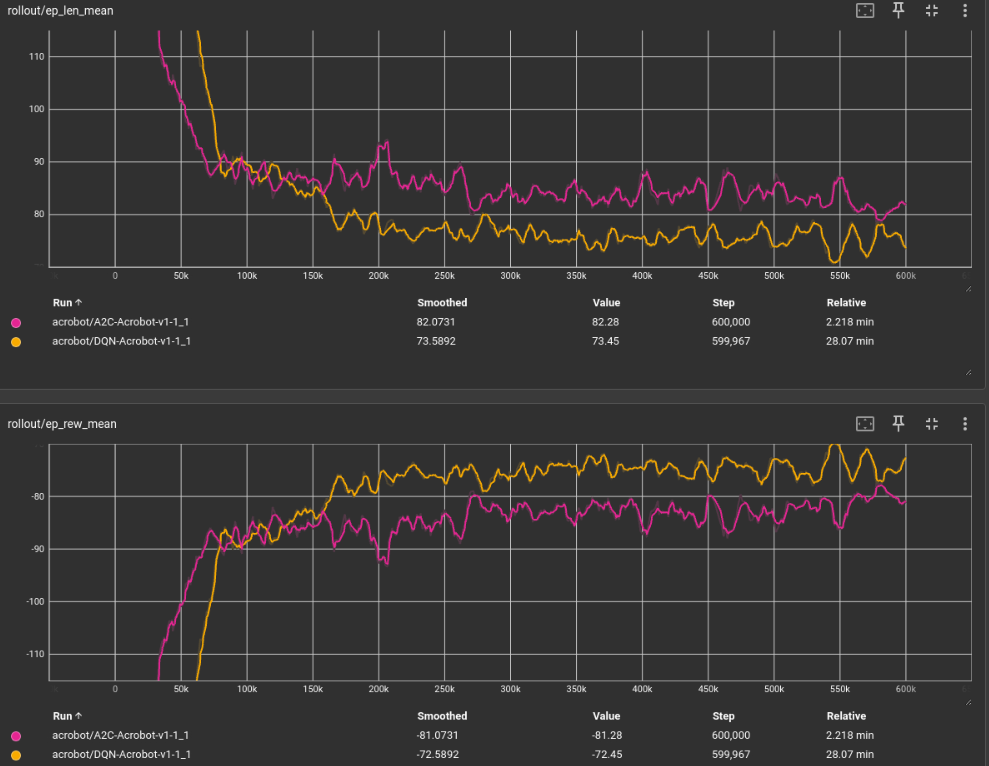
\includegraphics[width=7cm]{figs/Plataformas_Desarollo/TensorBoard.png}
  \end{center}
  \caption{Visualización de datos en TensorBoard.}
  \label{tensorboard}
\end{figure}

\section{Entornos de desarrollo}
\label{sec:des}

\subsection{Anaconda}
\label{sec:conda}

Anaconda \footnote{\url{https://www.anaconda.com/}} es una plataforma de distribución de software que facilita la gestión de entornos y librerías para el desarrollo de aplicaciones en Python. Permite crear entornos aislados con versiones específicas de Python y otras dependencias, lo que ayuda a evitar conflictos entre proyectos y a garantizar que las aplicaciones se ejecuten con las versiones requeridas de las bibliotecas. En este \ac{TFG}, se crea un entorno Anaconda que nos permita utilizar la versión 3.10 de Python, ya que es la que necesitaremos para utilizar EfficientVit.

\begin{code}[h]
\begin{lstlisting}[language=bash]

conda create -n tfg python=3.10
conda activate tfg

\end{lstlisting}
\caption[Creación del entorno Anaconda]{Creación y activación del entorno Anaconda.}
\label{cod:anaconda}
\end{code}

\subsection{Visual Studio Code}
\label{sec:vs_code}

Visual Studio Code \footnote{\url{https://code.visualstudio.com/}} es un editor de código gratuito y compatible con varias plataformas, diseñado para crear, modificar y depurar código en varios lenguajes de programación. Este software también incluye herramientas adicionales como extensiones que optimizan la escritura en diferentes lenguajes, autocompletado de código y terminales integrados para hacer más eficiente la ejecución y depuración.

\begin{figure}[ht]
  \begin{center}
    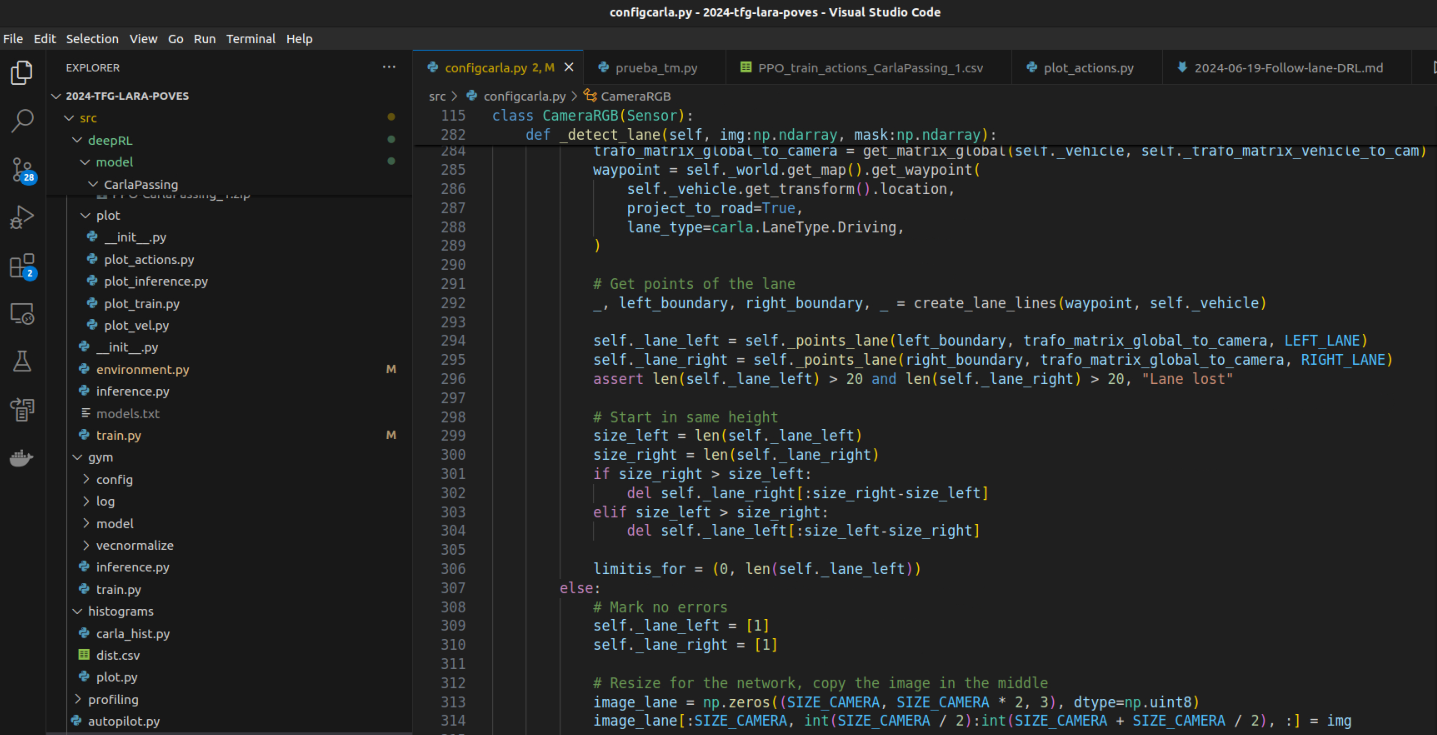
\includegraphics[width=10cm]{figs/Plataformas_Desarollo/visual_code.png}
  \end{center}
  \caption{Desarrollo en Visual Studio Code.}
  \label{foto_code}
\end{figure}

\newpage

En este \ac{TFG}, se utiliza Visual Studio Code como el editor principal para el desarrollo de todo el código, aprovechando sus extensiones para Python y YAML \footnote{\url{https https://www.ibm.com/es-es/topics/yaml}}, lo cual optimizó la productividad y facilitó la escritura del código.

\section{Herramientas para la detección de carril}
\label{sec:herramientas_carril}

Para la detección de carril, se ha utilizado la herramienta \textit{carla\_lane\_detector}, desarrollada por RoboticsLabURJC. Esta herramienta permite identificar con precisión las líneas que delimitan el carril dentro del simulador CARLA, proporcionando información crucial para el control y la navegación del vehículo autónomo, lo que permite además ajustar su trayectoria en función de la información obtenida. Existen dos técnicas principales para llevar a cabo esta detección: una basada en \ac{DL} y otra en información de CARLA.

\subsection{Detección \ac{DL}}
\label{sec:carril_dl3}

El modelo basado en \ac{DL} ha sido entrenado con imágenes tomadas del simulador CARLA y se ha implementado utilizando la librería PyTorch \footnote{\url{https://pytorch.org/}}. Este modelo de segmentación está diseñado para identificar las líneas del carril en entornos simulados, aprendiendo patrones a partir de un conjunto amplio de datos y generando una máscara que indica la probabilidad de que cada píxel pertenezca a una de las líneas de carril. Sin embargo, este enfoque presenta algunas limitaciones, por ejemplo, si un vehículo está delante y oculta las líneas del carril, el modelo no es capaz de resolver esta situación, lo que podría llevar a una detección del carril imprecisa o incluso nula.

\begin{figure}[ht]
  \begin{center}
    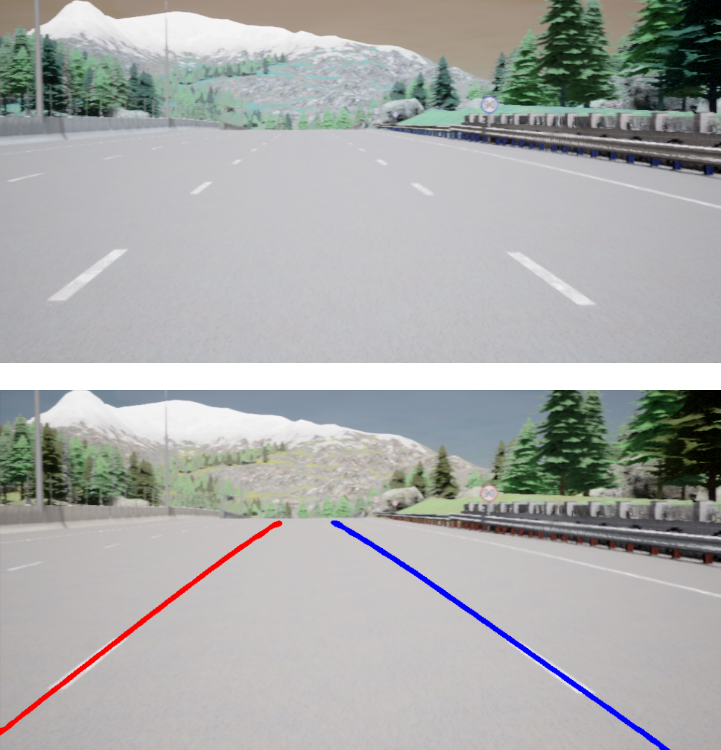
\includegraphics[width=6cm]{figs/Plataformas_Desarollo/carla_lane_dl.png}
  \end{center}
  \caption{Detección de carril basada en \ac{DL}.}
  \label{dl_lane}
\end{figure}

\subsection{Detección ground truth}
\label{sec:gt}

Por otro lado, la detección de carril basada en \textit{ground truth} aprovecha la ubicación del vehículo y la cámara dentro de CARLA para realizar la detección del carril. Gracias a la transformación de coordenadas entre el vehículo y la cámara, junto con la posición precisa del vehículo, es posible obtener los límites del carril en 3D, visión global en CARLA. Además, disponemos de la matriz intrínseca K, que permite la conversión de coordenadas de 2D a 3D. Utilizando esta matriz, los límites del carril pueden proyectarse a 2D. A diferencia de la solución basada en \ac{DL}, este enfoque no depende de la visibilidad directa de las líneas del carril, si hay elementos que obstruyen la visión, la detección sigue siendo precisa, ya que se basa en información global del entorno de CARLA y no en una imagen.

\begin{figure}[ht]
  \begin{center}
    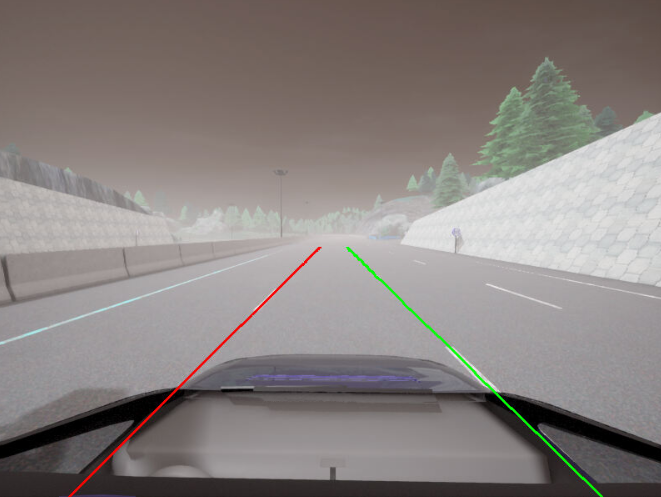
\includegraphics[width=7cm]{figs/Plataformas_Desarollo/ground_truth.png}
  \end{center}
  \caption{Detección de carril basada en \textit{ground truth}.}
  \label{dl_lane}
\end{figure}

\section{EfficientVit}
\label{sec:ef}

EfficientViT es un innovador módulo dentro de la familia de \textit{Vision Transformers} \footnote{\url{https://arxiv.org/pdf/1706.03762}}, utilizado con éxito en tareas como segmentación semántica, superresolución de imágenes y modelos de segmentación generalizados. Su principal ventaja es la significativa reducción de latencias sin perder rendimiento, haciendo posible su uso en aplicaciones de tiempo real. A diferencia de los modelos tradicionales que dependen de mecanismos de atención computacionalmente costosos o convoluciones de gran tamaño, EfficientViT emplea una atención lineal multiescala \footnote{\textbf{Multiescala:} enfoque que procesa información en distintos niveles de detalle simultáneamente para mejorar la eficiencia y precisión} ligera \cite{efficientvit}.

La segmentación es el proceso de dividir una imagen en regiones significativas para identificar objetos y se divide en dos tipos principales: segmentación semántica y segmentación de instancias. En la segmentación semántica, se asigna una clase a cada píxel de la imagen, pero no se distingue entre diferentes instancias de una misma clase. En cambio, la segmentación de instancias, no solo clasifica los píxeles en categorías, sino que también identifica y distingue las instancias individuales de un objeto. Por ejemplo, en una imagen con varios vehículos, la segmentación de instancias, además de clasificar los píxeles como vehículos, es capaz de diferenciar entre cada vehículo de forma individual.

En este \ac{TFG}, se utiliza el modelo EfficientViT Segmentation \footnote{\url{ https://github.com/mit-han-lab/efficientvit/blob/master/applications/efficientvit_seg}} para detectar la calzada. Este modelo ha sido entrenado con \textit{Cityscapes Dataset} \footnote{\url{https://www.cityscapes-dataset.com/}}, diseñado para la comprensión semántica de escenas urbanas, centrándose en la segmentación de calles y objetos en entornos urbanos. Este \textit{dataset} incluye anotaciones poligonales, que marcan con precisión los objetos en las imágenes realizando una segmentación semántica densa, asignando una etiqueta a cada píxel de la imagen. Además, para objetos como vehículos y personas, se emplea segmentación de instancias.

\begin{figure}[ht]
\begin{center}
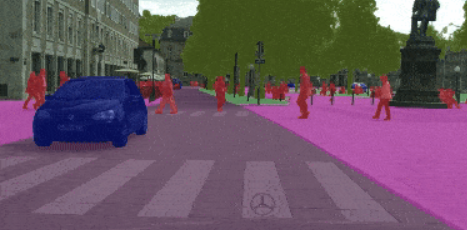
\includegraphics[width=7cm]{figs/Plataformas_Desarollo/resultado_ef.png}
\end{center}
\caption{Resultado de segmentación semántica con EfficientViT \cite{efficientvit-gif}.}
\label{foto_ef}
\end{figure}

Este conjunto de datos contiene imágenes reales tomadas en 50 ciudades durente diferentes estaciones del año, condiciones meteorológicas variadas y a distintas horas del día. Las imágenes fueron seleccionadas manualmente, asegurando una gran cantidad de objetos dinámicos, así como variación en el fondo y en la disposición de las escenas. \textit{Cityscapes Dataset} incluye un total de 5.000 imágenes con anotaciones detalladas y 20.000 con anotaciones más generales, cubriendo 30 clases de objetos urbanos. Esto lo convierte en un recurso muy útil para entrenar modelos de visión por computadora en entornos urbanos con muchos elementos.
\begin{figure}[ht]
\begin{center}
% Imagen con datos detallados del dataset
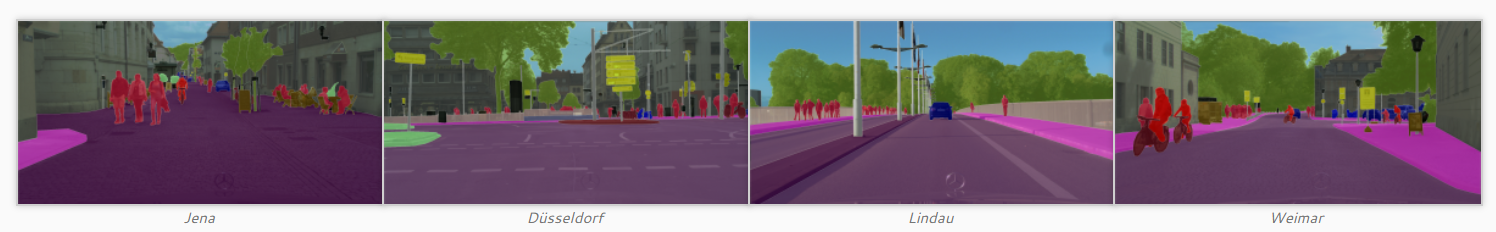
\includegraphics[width=15cm]{figs/Plataformas_Desarollo/detallado-ef.png}
\caption{Ejemplo de imagen con datos detallados de \textit{Cityscapes Dataset} \cite{cityscapes}.}
\label{foto_ef_detallado}
\vspace{0.5cm} % Espacio entre las dos imágenes
% Imagen con datos más generales del dataset
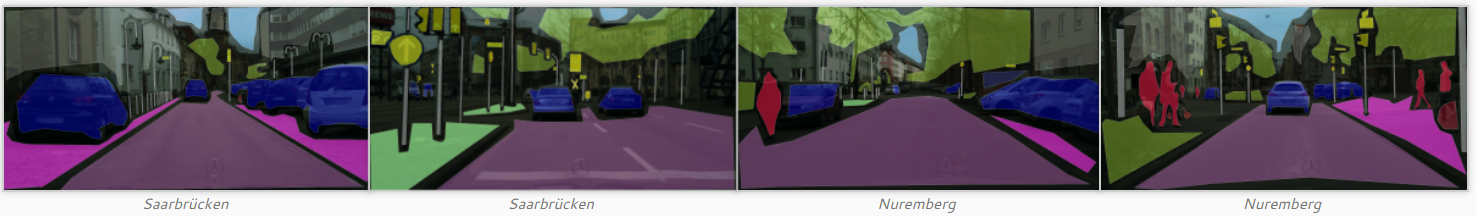
\includegraphics[width=15cm]{figs/Plataformas_Desarollo/no_detallado_ef.png}
\caption{Ejemplo de imagen con datos más generales de \textit{Cityscapes Dataset} \cite{cityscapes}.}
\label{foto_ef_general}
\end{center}
\end{figure}

\section{Entorno de simulación}
\label{sec:sim}
\subsection{CARLA}
\label{sec:carla}

CARLA \footnote{\url{https://github.com/carla-simulator/carla}} es un entorno de simulación de código abierto que se emplea en aplicaciones de conducción autónoma. CARLA se basa en \textit{Unreal Engine de Epic Games} \footnote{\url{https://www.unrealengine.com/en-US}}, lo que le permite generar entornos urbanos y rurales altamente detallados y realistas. Estos entornos son ideales para simular la interacción de los vehículos autónomos con el entorno, probando su capacidad de navegación, toma de decisiones y respuesta ante situaciones imprevistas.

\begin{code}[h]
\begin{lstlisting}[language=bash]

/opt/carla/CarlaUE4.sh -world-port=2000

\end{lstlisting}
\caption[Comando para lanzar el simulador CARLA]{Comando para lanzar el simulador CARLA.}
\label{cod:cmdcarla}
\end{code}

Este simulador destaca por su capacidad de recrear escenarios dinámicos con una amplia variedad de condiciones de tráfico, clima y paisajes urbanos, convirtiéndolo en una herramienta valiosa para la investigación en condiciones similares a las del mundo real. Para aprovechar estos entornos, utilizaremos \textit{scripts} de Python que nos permitirán personalizar las simulaciones, brindando flexibilidad para ajustar propiedades como el comportamiento de los vehículos o la configuración de los sensores.

\begin{figure}[ht]
\begin{center}
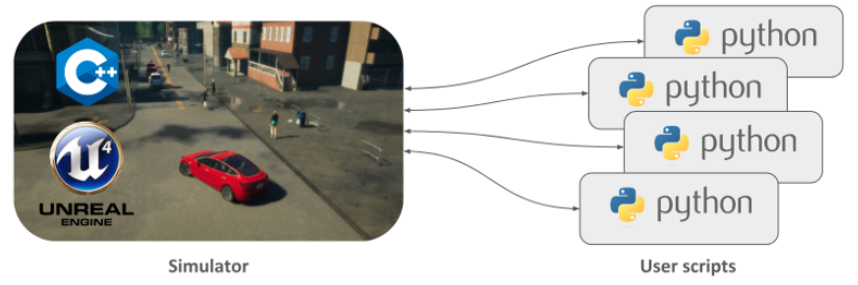
\includegraphics[width=9cm]{figs/Plataformas_Desarollo/carla.png}
\end{center}
\caption{Simulador CARLA.}
\label{carla}
\end{figure}

En CARLA, los mapas son modelos tridimensionales detallados de ciudades y sus infraestructuras viales, que no solo incluyen la geometría de las carreteras y edificios, sino también objetos interactivos como semáforos, señales de tráfico y otros elementos estáticos, los cuales pueden activarse o desactivarse según las necesidades del usuario. CARLA ofrece una amplia selección de mapas predefinidos que se pueden cargar directamente. Por otro lado, el mundo en CARLA se refiere al entorno completo de la simulación, que incluye el mapa, el clima, el tiempo, los vehículos, los peatones y otros elementos dinámicos, permitiendo crear una simulación realista y modificable en tiempo real para ajustar factores como la hora del día, las condiciones climáticas o el tráfico.

\subsubsection{Actores}

Los actores en CARLA son los elementos que realizan acciones dentro de la simulación y pueden interactuar con otros actores. Existen varios tipos de actores, cada uno con funcionalidades específicas:

\begin{itemize}
\item \textit{Sensores.} Los sensores \footnote{\url{https://carla.readthedocs.io/en/latest/core_sensors/}} son actores capaces de producir un flujo de datos y existen diversos tipos disponible. La mayoría de los sensores se anexan a un vehículo para recopilar información sobre su entorno, indicando la localización y rotación respecto al mismo. Los sensores escuchan datos y, cuando reciben información, llaman a una función descrita mediante una expresión \textit{Lambda} \footnote{\url{https://docs.python.org/3/reference/expressions.html}}. 

	\begin{code}[h]
	\begin{lstlisting}[language=python]
	
	camera_bp = blueprint_library.find('sensor.camera.rgb')
	camera = world.spawn_actor(camera_bp, transform, attach_to=vehicle)
	camera.listen(lambda image: image.save_to_disk('output/%06d.png' % image.frame))

	\end{lstlisting}
	\caption[Configuración de cámara RGB en CARLA]{Configuración de cámara RGB en CARLA.}
	\label{cod:camara_carla}
	\end{code}


\item \textit{Espectador.} El espectador proporciona un punto de vista dentro de la simulación. Puede utilizarse para mover la vista en la ventana del simulador.
\item \textit{Señales de tráfico y semáforos.} En CARLA, solo las señales de \textit{stop}, ceda el paso y los semáforos son considerados actores.

\item \textit{Vehículos.} Los vehículos en CARLA son un tipo especial de actor que simula la física de los vehículos de ruedas real. Utilizan un controlador que define los atributos físicos del vehículo y otro que gestiona los comandos de conducción: aceleración, dirección y freno. CARLA ofrece varios tipos de vehículos (coches, motocicletas y camiones... \footnote{\url{https://carla.readthedocs.io/en/latest/catalogue_vehicles/}}), además de una gran variedad de modelos. El vehículo que se desea controlar, al que se le añaden los sensores, conocido como \textit{Ego Vehicle}, será el agente en el proceso de aprendizaje. Si indicamos esta condición al simulador, este renderiza solo la zona cercana a este vehículo para optimizar recursos.

	\begin{code}[h]
	\begin{lstlisting}[language=python]
	
	vehicle_vp = world.get_blueprint_library().find(vehicle_type)
	vehicle_vp.set_attribute('role_name', 'hero') # Ego vehicle
	ego_vehicle = world.spawn_actor(vehicle_bp, transform)
	ego_vehicle.apply_control(carla.VehicleControl(throttle=0.5, steer=0.1, brake=0.01))

	\end{lstlisting}
	\caption[Configuración de \textit{Ego Vehicle} en CARLA]{Configuración de \textit{Ego Vehicle} en CARLA.}
	\label{cod:ego_carla}
	\end{code}
    \item \textit{Peatones.} Los peatones funcionan de manera similar a los vehículos. El control sobre ellos se proporciona mediante controladores.
\end{itemize}

En este \ac{TFG} se utiliza como \textit{Ego Vehicle} el modelo \textit{Lincoln MKZ 2020} \footnote{\url{https://carla.readthedocs.io/en/latest/catalogue_vehicles/\#lincoln-mkz-2020}}, sobre el cual solo se controlarán los actuadores de giro y aceleración. El acelerador (\textit{throttle}) tiene un rango de 0 a 1, mientras que el giro (\textit{steer}) varía entre -1 y 1, donde -1 es giro a la izquierda y 1 a la derecha. Para simular el tráfico, se emplea un camión \footnote{\url{https://carla.readthedocs.io/en/latest/catalogue_vehicles/\#carla-motors-carlacola}} controlado por el autopiloto de CARLA, ya que, al no contar con cristales en la parte trasera, facilita la detección mediante el \ac{LiDAR}.

Al vehículo principal se le añaden tres tipos de sensores:

\begin{itemize}
\item \textit{Detector de colisión} \footnote{\url{https://carla.readthedocs.io/en/latest/ref_sensors/\#collision-detector}}. Este sensor registra un evento cada vez que el vehículo colisiona con un objeto en el entorno. Para identificar contra qué vehículo se ha chocado, se debe consultar el atributo \textit{other\_actor} en los datos del sensor.

\item \textit{Cámara RGB} \footnote{\url{https://carla.readthedocs.io/en/latest/ref_sensors/\#rgb-camera}}. La cámara RGB actúa como una cámara convencional, capturando imágenes de la escena. Se pueden configurar distintos parámetros, como las dimensiones de la imagen y el campo de visión. En este caso, se establecen dimensiones de 512 × 512 píxeles para garantizar compatibilidad con EfficientVit. Para consultar la matriz que define la imagen, debemos mirar en los datos de salida el atributo \textit{raw\_data}.

\item \textit{Sensor \ac{LiDAR}} \footnote{\url{https://carla.readthedocs.io/en/latest/ref_sensors/\#lidar}}. Este sensor simula un \ac{LiDAR} rotativo mediante \textit{ray-casting}, generando puntos al agregar un \ac{LiDAR} por cada canal distribuido en el campo visual vertical. Los datos se codifican en cuatro dimensiones: las primeras tres corresponden a la posición en \textit{x, y, z}, y la cuarta representa la intensidad de la señal reflejada. Se pueden configurar parámetros como los ángulos del campo de visión superior, inferior y horizontal, siendo en nuestro caso un láser de 360º, mientras que el resto de los atributos se mantienen con los valores por defecto. Además, es posible ajustar la frecuencia de rotación y la cantidad de puntos por segundo, lo cual adaptaremos dependiendo de los \ac{FPS} alcanzados. Al igual que en la cámara, los datos de salida incluyen la nube de puntos completa en el atributo \textit{raw\_data}.
\end{itemize}

\subsubsection{Traffic Manager}

El \ac{TM} es el módulo encargado de controlar los vehículos en modo piloto automático dentro de una simulación. Su propósito principal es recrear condiciones de tráfico urbano realistas en el entorno simulado. Los usuarios tienen la posibilidad de personalizar ciertos comportamientos para configurar escenarios específicos de aprendizaje, para simular diferentes circunstancias de conducción.

El \ac{TM} está integrado en el lado cliente de CARLA, y es necesario especificar el puerto de conexión para su funcionamiento. Los usuarios pueden ajustar parámetros del flujo de tráfico, permitiendo, forzando o incentivando comportamientos específicos. Por ejemplo, se puede configurar que los vehículos ignoren los límites de velocidad, cambien de carril de forma obligatoria o adopten comportamientos personalizados. Estas capacidades permiten experimentar y simular situaciones para el entrenamiento y evaluación de sistemas de conducción autónoma.

En nuestro caso, los entrenamientos estarán limitados al uso del autopiloto para el coche delantero con una velocidad fija e ignorando completamente las señales de tráfico para realizar el control adaptativo el tráfico y el adelantamiento. 

\begin{code}[h]
	\begin{lstlisting}[language=python]
	
	tm = client.get_trafficmanager(port)
	vehicle.set_autopilot(True, tm.get_port())  
	tm.ignore_lights_percentage(vehicle, 100) 
	self._tm.set_desired_speed(vehicle, velocity) #km/h
\end{lstlisting}
\caption[Configuración del \textit{Traffic Manager} en CARLA]{Configuración del \textit{Traffic Manager} en CARLA.}
\label{cod:tm_carla}
\end{code}

\section{Hardware}
\label{sec:hw}
\subsection{Servidor Thor}
\label{sec:thor}

CARLA es un simulador que requiere una gran capacidad computacional. La ejecución de algoritmos de aprendizaje por refuerzo, combinados con diversas redes neuronales para la percepción, incrementa aún más esta demanda de potencia. Para satisfacer estos requisitos, es fundamental disponer de los recursos de hardware adecuados. Lo ideal es contar con una o varias \ac{GPU}, ya que están optimizadas para el procesamiento paralelo masivo, lo que en nuestro caso aceleraría significativamente tanto la simulación como el entrenamiento de modelos de \ac{IA}. 

El servidor Thor, ubicado en la Escuela de Ingeniería Superior de Fuenlabrada de la \ac{URJC}, forma parte de la granja de servidores con \ac{GPU} de RoboticsLabURJC. Este servidor está diseñado para tareas que requieren un alto rendimiento, ya que su arquitectura \textit{x86\_64} y el potente procesador \textit{AMD Ryzen Threadripper 7960X} lo hacen adecuado para aplicaciones exigentes. La velocidad del procesador varía dependiendo de la carga de trabajo, oscilando entre 545 MHz en reposo y hasta 7786 MHz cuando se necesita el máximo rendimiento, lo que contribuye tanto a la optimización del consumo energético como a la mejora del desempeño del sistema. En cuanto al almacenamiento, el servidor cuenta con 125 GiB de memoria \ac{RAM} y su capacidad total de disco es de 24,8 TB, distribuida entre las diferentes unidades de almacenamiento.

Además, el servidor está equipado con una \ac{GPU} NVIDIA GeForce RTX 4090 con 24 GB de memoria, lo que permite no solo gestionar cargas computacionales intensivas, sino también facilitar el entrenamiento y la inferencia de modelos en tiempo real. Esta capacidad es crucial para el desarrollo y las pruebas de este \ac{TFG}, como se puede observar en la Figura \ref{fig:thor_nvidia}.

\begin{figure}[ht]
  \centering
  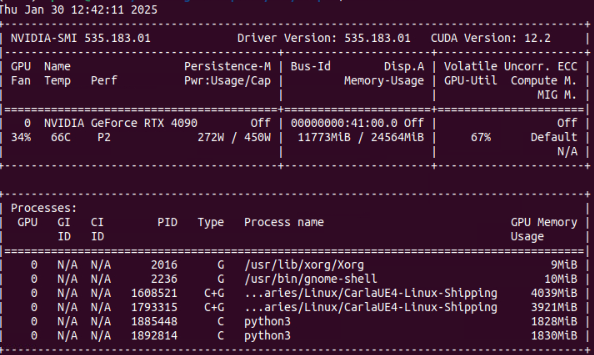
\includegraphics[width=9cm]{figs/Plataformas_Desarollo/thor.png}
  \caption{Servidor Thor equipado con una \ac{GPU}.}
  \label{fig:thor_nvidia}
\end{figure}









